\documentclass{article}

%\usepackage[margin=2.54cm]{geometry}
\usepackage{setspace}

\usepackage[british]{babel}
\usepackage{csquotes}
\usepackage{hyperref}

\usepackage[backend=biber,style=alphabetic]{biblatex}
\addbibresource{\jobname.bib}

\usepackage{acronym}
\acrodef{ACT}{auto-correlation time}
\acrodef{ESS}{effective sample size}
\acrodef{HMC}{Hamiltonian Monte Carlo}
\acrodef{MCMC}{Markov chain Monte Carlo}
\acrodef{ODE}{ordinary differential equation}

\usepackage{mathtools}
\newcommand{\dd}{\, \mathrm{d}}
\renewcommand{\vec}[1]{\ensuremath{\boldsymbol{\mathbf{#1}}}}
\newcommand{\mat}[1]{\ensuremath{\boldsymbol{\mathbf{#1}}}}
\newcommand{\op}[1]{\ensuremath{\boldsymbol{\mathbf{#1}}}}
\newcommand{\norm}[1]{\ensuremath{\mathcal{N}\left(#1\right)}}

\usepackage{algorithm}
\usepackage{algpseudocode}

\usepackage{graphicx}
\usepackage{caption}
\usepackage{subcaption}
\captionsetup[ruled]{labelsep=period}

\title{Implementing \acl{HMC} for Efficient Bayesian Evolutionary Analysis \\
           \Large\textsc{awc summer scholarship report}}
\author{Arman Bilge \\ \texttt{\href{mailto:armanbilge@gmail.com}{armanbilge@gmail.com}}}
\date{23 April 2015}

\frenchspacing
\begin{document}

    \maketitle

    \subsection*{Introduction}
    In September 2014 I proposed a project that compared the performance of the
        \ac{HMC} algorithm~\cite{Dua+87,Nea11} to that of the
        Metropolis--Hastings \ac{MCMC} algorithm~\cite{Met+53,Has70} in the
        context of Bayesian evolutionary analysis.
    This project was largely motivated by theoretical results that suggested
        that \ac{HMC} scales better than \ac{MCMC} as problem size increases.
    Specifically, \textcite{Nea11} showed that for a problem in $n$~dimensions,
        the computation time required for a given level of accuracy is
        proportional to $n^\frac{5}{4}$ for \ac{HMC} and to $n^2$ for
        \ac{MCMC}.
    To arrive at this result, we must assume that the $n$~variables are
        independent and that evaluating the target probability density or its
        partial derivative takes a single time unit.
    I will adjust the latter of these assumptions to show that \ac{HMC} does
        not scale better than \ac{MCMC} in the context of Bayesian evolutionary
        analysis.
    This result is supported by practical experiments.

    At the core of a Bayesian evolutionary analysis is a distribution of
        phylogenetic trees~\cite{Bou+14}, given by the product of the
        Felsenstein likelihood~\cite{Fel81} and an arbitrary prior.
    If we condition on the tree structure, then we have a distribution on edge
        weights (interpreted as branch lengths).
    Evaluating the Felsenstein likelihood involves a post-order traversal where
        likelihoods at each internal node depend on the likelihoods of its
        children and the weights of the edges connecting them; the likelihoods
        at leaf nodes are given directly by the data.
    These partial likelihoods at each node may be cached and reused so long as
        their dependencies are not updated.
    Evaluating the partial derivative of the Felsenstein likelihood with
        respect to an edge weight forces recalculation at all nodes ancestral
        to that edge; however, the cached partial likelihoods at all other
        nodes may be reused for differentiation.
    I will consider partial calculation at a single node as the primitive
        operation for my analysis of the algorithms.

    \subsection*{Main Result}

    Consider a full binary tree with $n$ edges.
    If all of the edge weights are updated then evaluating the Felsenstein
        likelihood requires recalculating partials at the $n$ internal nodes
        for a total of $n$ operations.
    \textcite{Nea11} showed that

    \subsection*{Discussion}

    \begin{figure}
        \centering
        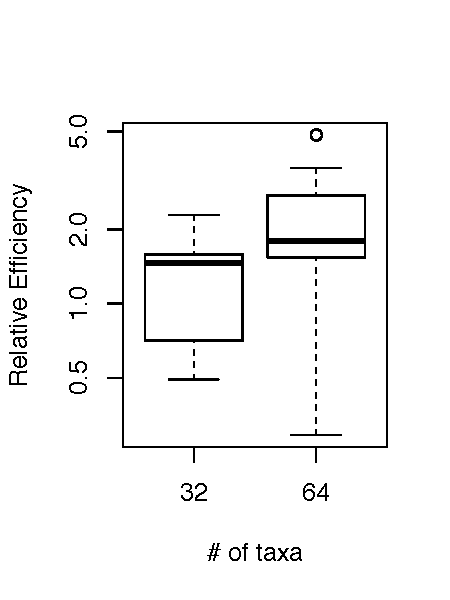
\includegraphics[scale=0.8]{boxplot.pdf}
        \caption{The efficiency of \ac{HMC} relative to \ac{MCMC} for simulated
                 datasets of 32, 64, and 128 taxa.}
    \end{figure}

    \printbibliography

\end{document}
